%! Author = ryan
%! Date = 12/25/21

% Preamble
\documentclass[11pt]{article}


% Packages
\usepackage{amsmath}
\usepackage[margin=1in]{geometry}
\usepackage{caption}
\usepackage{graphicx}
\usepackage{biblatex}

\addbibresource{ref.bib}


\title{Ising Simulations}
\author{Ryan T. Grimm}

% Document
\begin{document}

    \maketitle

\begin{abstract}
This document outlines a basic implementation of the two-dimensional Ising model coupled with a Metropolis Monte Carlo.
Initial results of the model show agreement with curves from literature, including heat capacity, magnetization, and magnetic susceptibility,
for a temperature sweep through a phase-transition with zero-field.
\end{abstract}


\section*{Binary Ising}
    We write the Hamiltonian of a two-dimensional ($N \times N$) spin-lattice with spins of $\sigma_{i}$ at site $i$ as
    \begin{align*}
        H _{\{\sigma_i\}}= \sum_{\langle i,j \rangle} J_{i,j} \sigma_i \sigma_j + \sum_i B_i \sigma_i,
    \end{align*} where $\langle i,j \rangle$ represent nearest neighbor pairs, $J$ is the coupling between sites, and $B$ is an external field.
    For this model, we assume that the field and couplings are uniform through the lattice.
    \begin{align*}
        H = J \sum_{\langle i,j \rangle} \sigma_i \sigma_j + B \sum_i \sigma_i,
    \end{align*}
    Additionally, we assume periodic boundary condition.

    The partition function in the canonical ensemble follows from the Hamiltonian.
    \begin{align*}
        Z = \sum_k \exp{\left(-\beta H_{\{\sigma_i\}}\right)}
    \end{align*}


    However, the system size grows like $2^{N \times N}$, which prohibits direct evaluation for non-trivial systems size.
    Thus, we employ Metropolis Monte Carlo to approximate a full enumeration of the configuration space of the lattice.
\section*{Metropolis}
The metropolis algorithm performs a random walk through configuration space while preserving detailed balance and Boltzmann distributed micro-states.
The outline of the algorithm is as follows.
    \begin{enumerate}
        \item Choose a random site $i$.
        \item Compute the change in energy, $\Delta E$, of site $i$ before and after a spin flip.
        \item If $\Delta E \leq 0$, accept the change.
        \item Otherwise, $\Delta E > 0$, accept the change with the probability $P = \exp(- \beta  \Delta E).$
    \end{enumerate} \\


    \begin{figure}
        \centering
        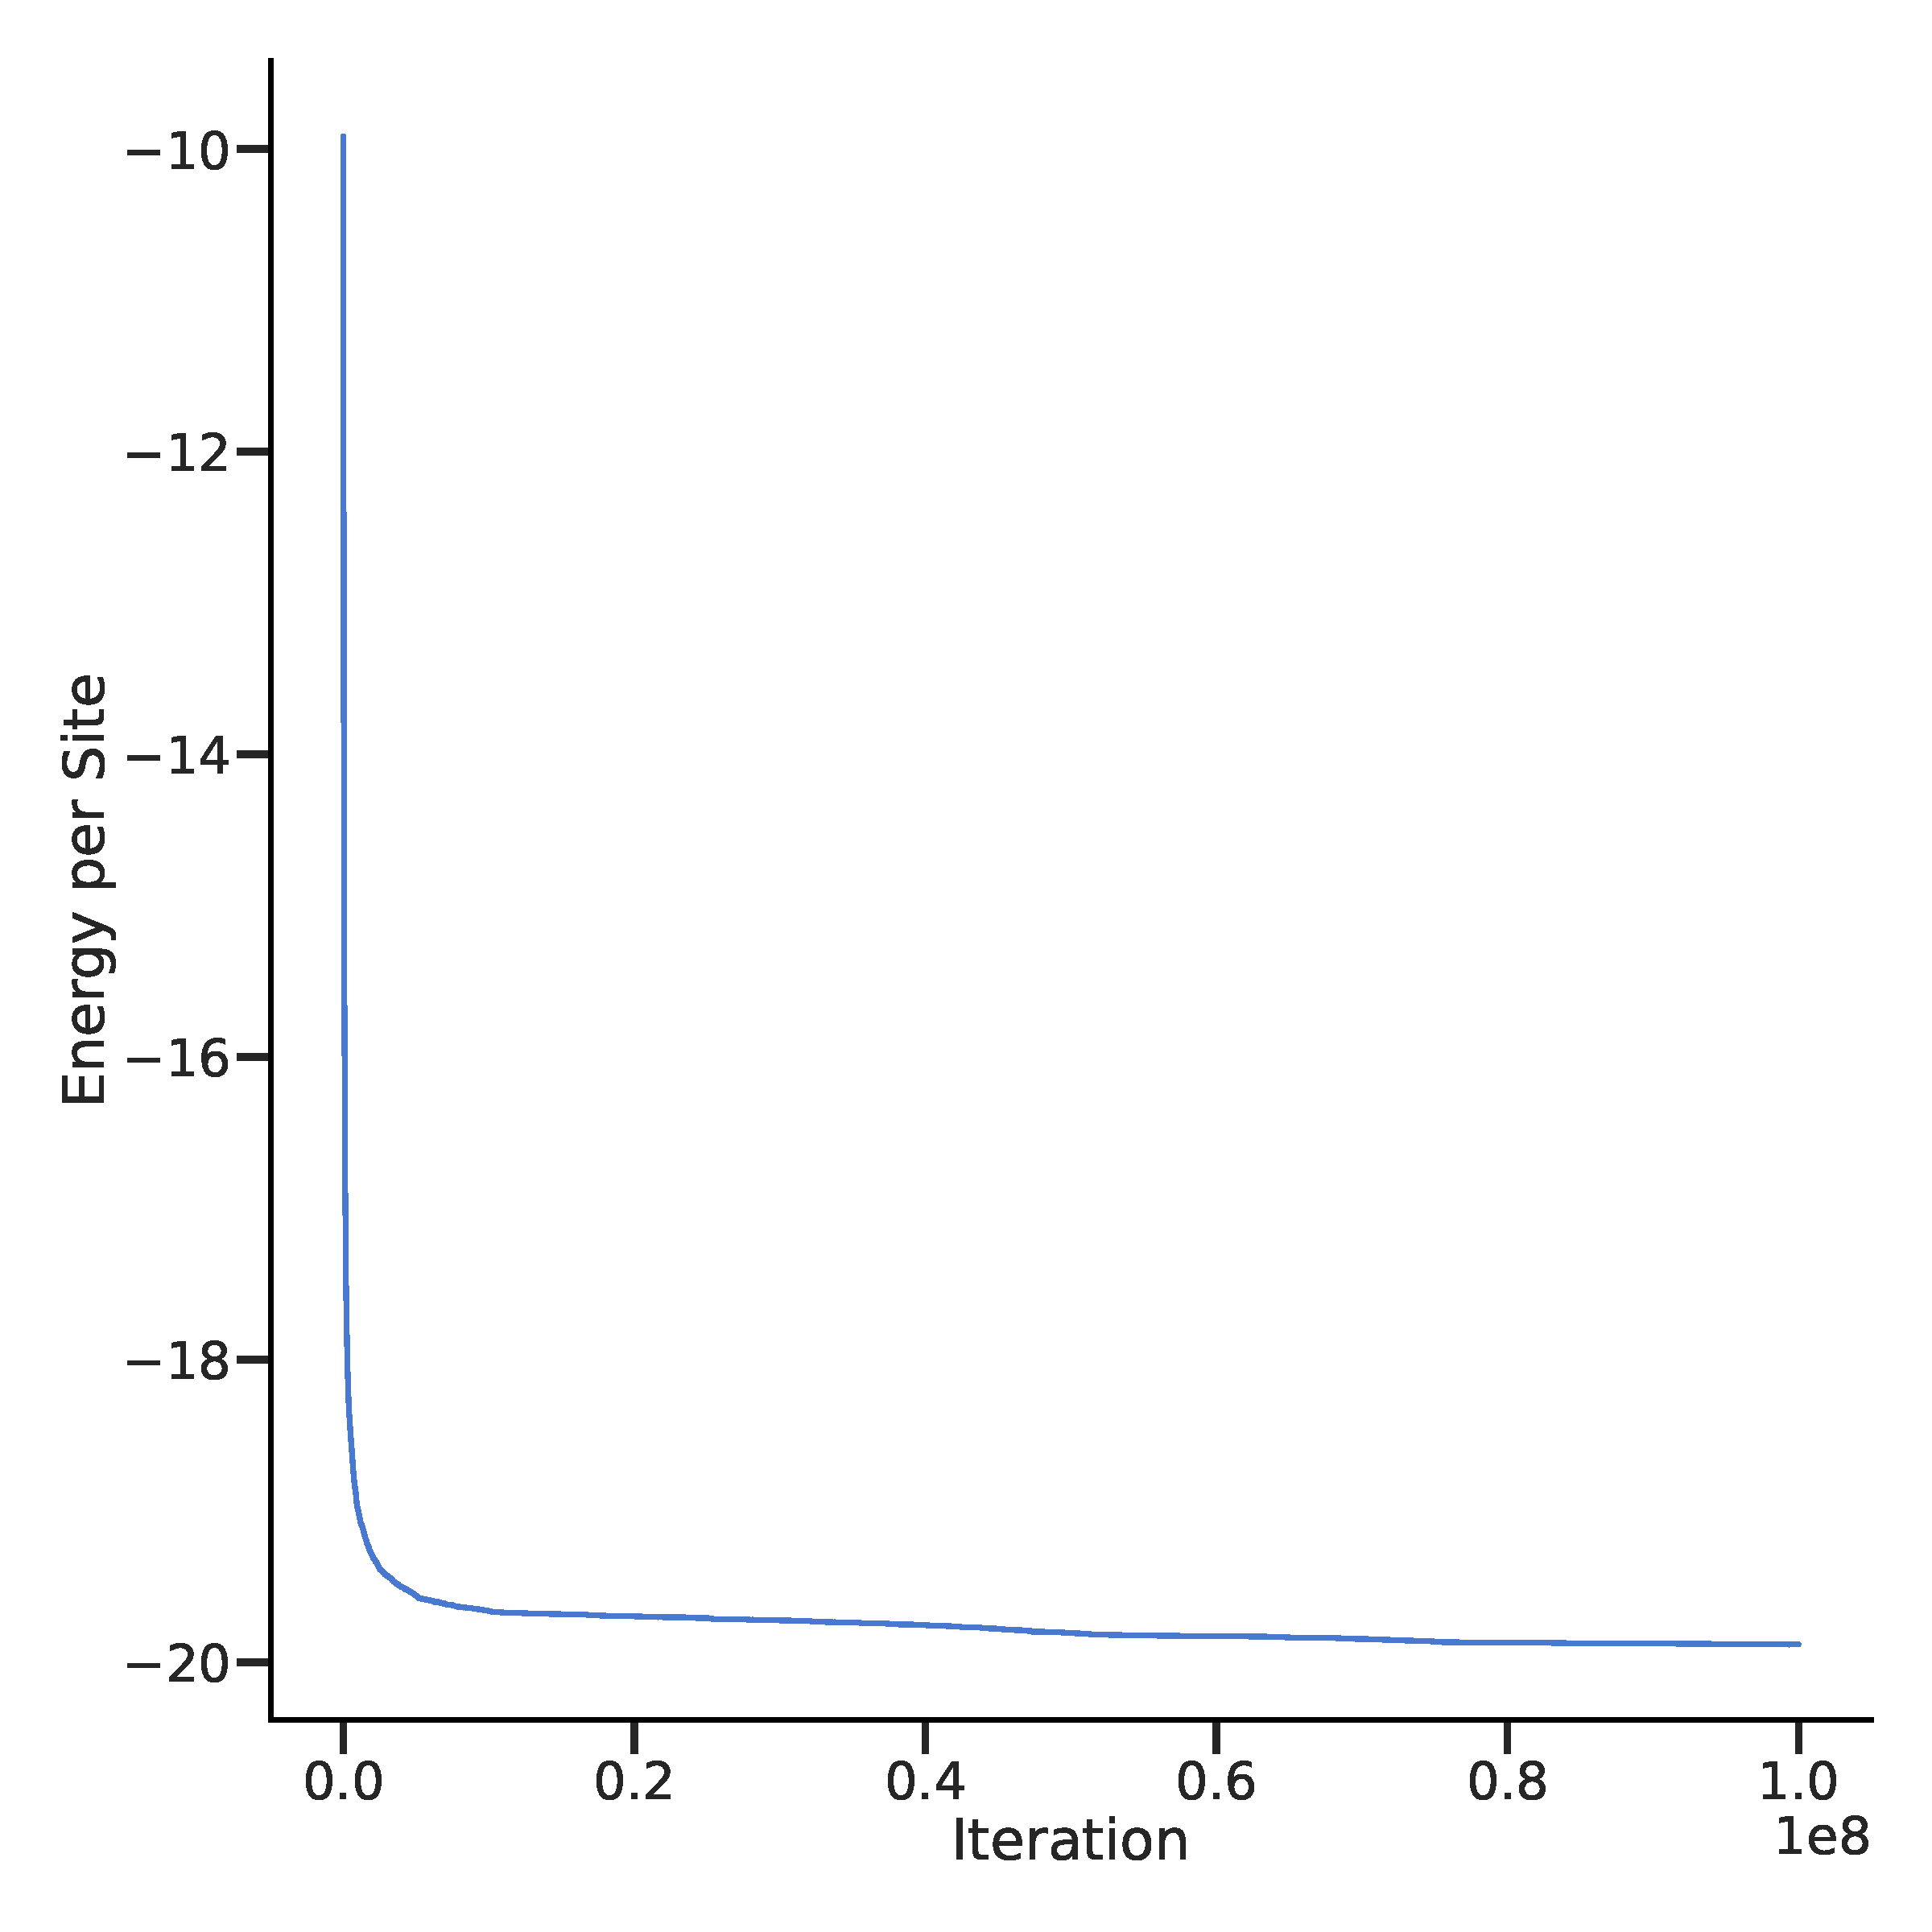
\includegraphics[width=0.6\textwidth]{../Python/eq.pdf}

        \caption{Equilibration of a $128 \times 128$ lattice. }
        \label{fig:eq}
    \end{figure}

First, the algorithm is run to attain an equilibrium configuration of the spin-lattice.
A sampling of a system's micro-states and fluctuations about equilibrium can then be obtained
by running Metropolis on the equilibrium configuration (Figure~\ref{fig:eq}).

    \newpage

\section*{Benchmarking \& Phase Transition}

    \begin{figure}
        \centering
        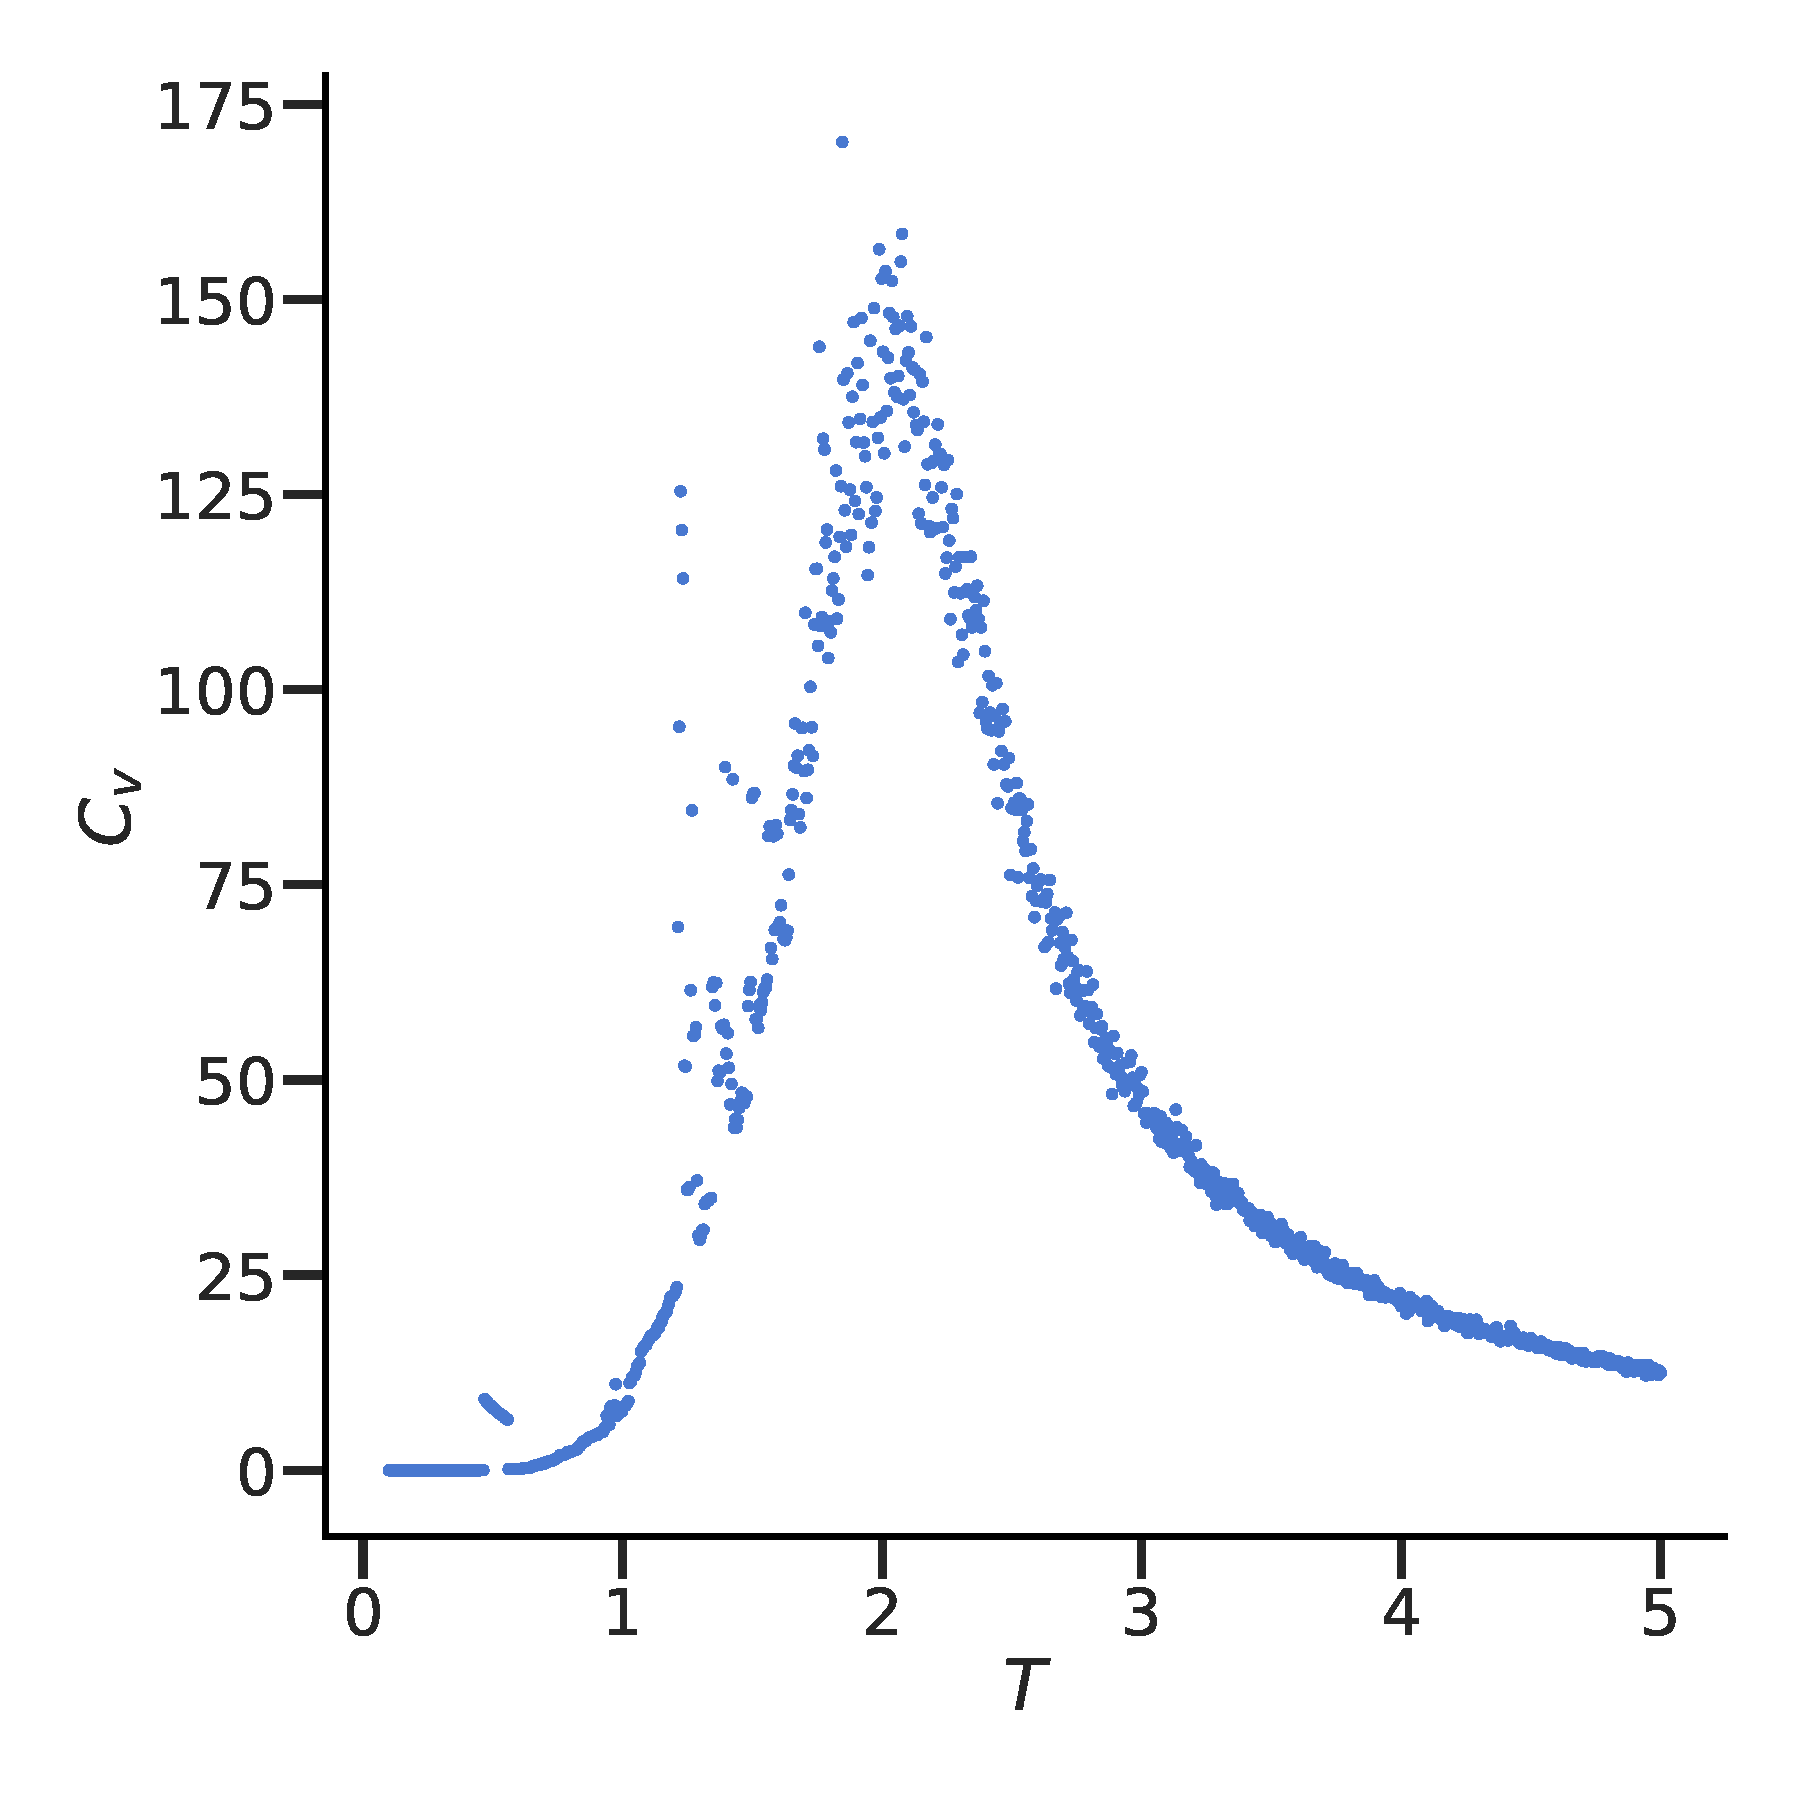
\includegraphics[width=0.6\textwidth]{../Python/heat_cap.pdf}

        \caption{Heat capacity as a function of temperature for a $12 \times 12$ lattice.}
        \label{fig:heat_cap}
    \end{figure}

    To test the validity of the model, a set of simulations were run over a range of temperatures
    - $0.1$ to $5.0$ (normalized units) - on a field-free ($B = 0$), $12 \times 12$ spin-lattice with $J = 1.0$.
    The heat capacity (Figure~\ref{fig:heat_cap}),
    expressed as
    \begin{align*}
        C_v = \frac{1}{k_b T^2}\left(\langle E^2 \rangle - \langle E \rangle^2)\right),
    \end{align*} exhibits a phase transition (as can be seen by the non-differentiability of $C_v(T)$ at its maximum) near the expected critical temperature, $T_c$, of 2.269.
    \begin{align*}
        T_c = \frac{J}{k_b} \frac{2}{\log{(1 + \sqrt {2})}} \approx 2.269
    \end{align*}

    \begin{figure}
        \centering
        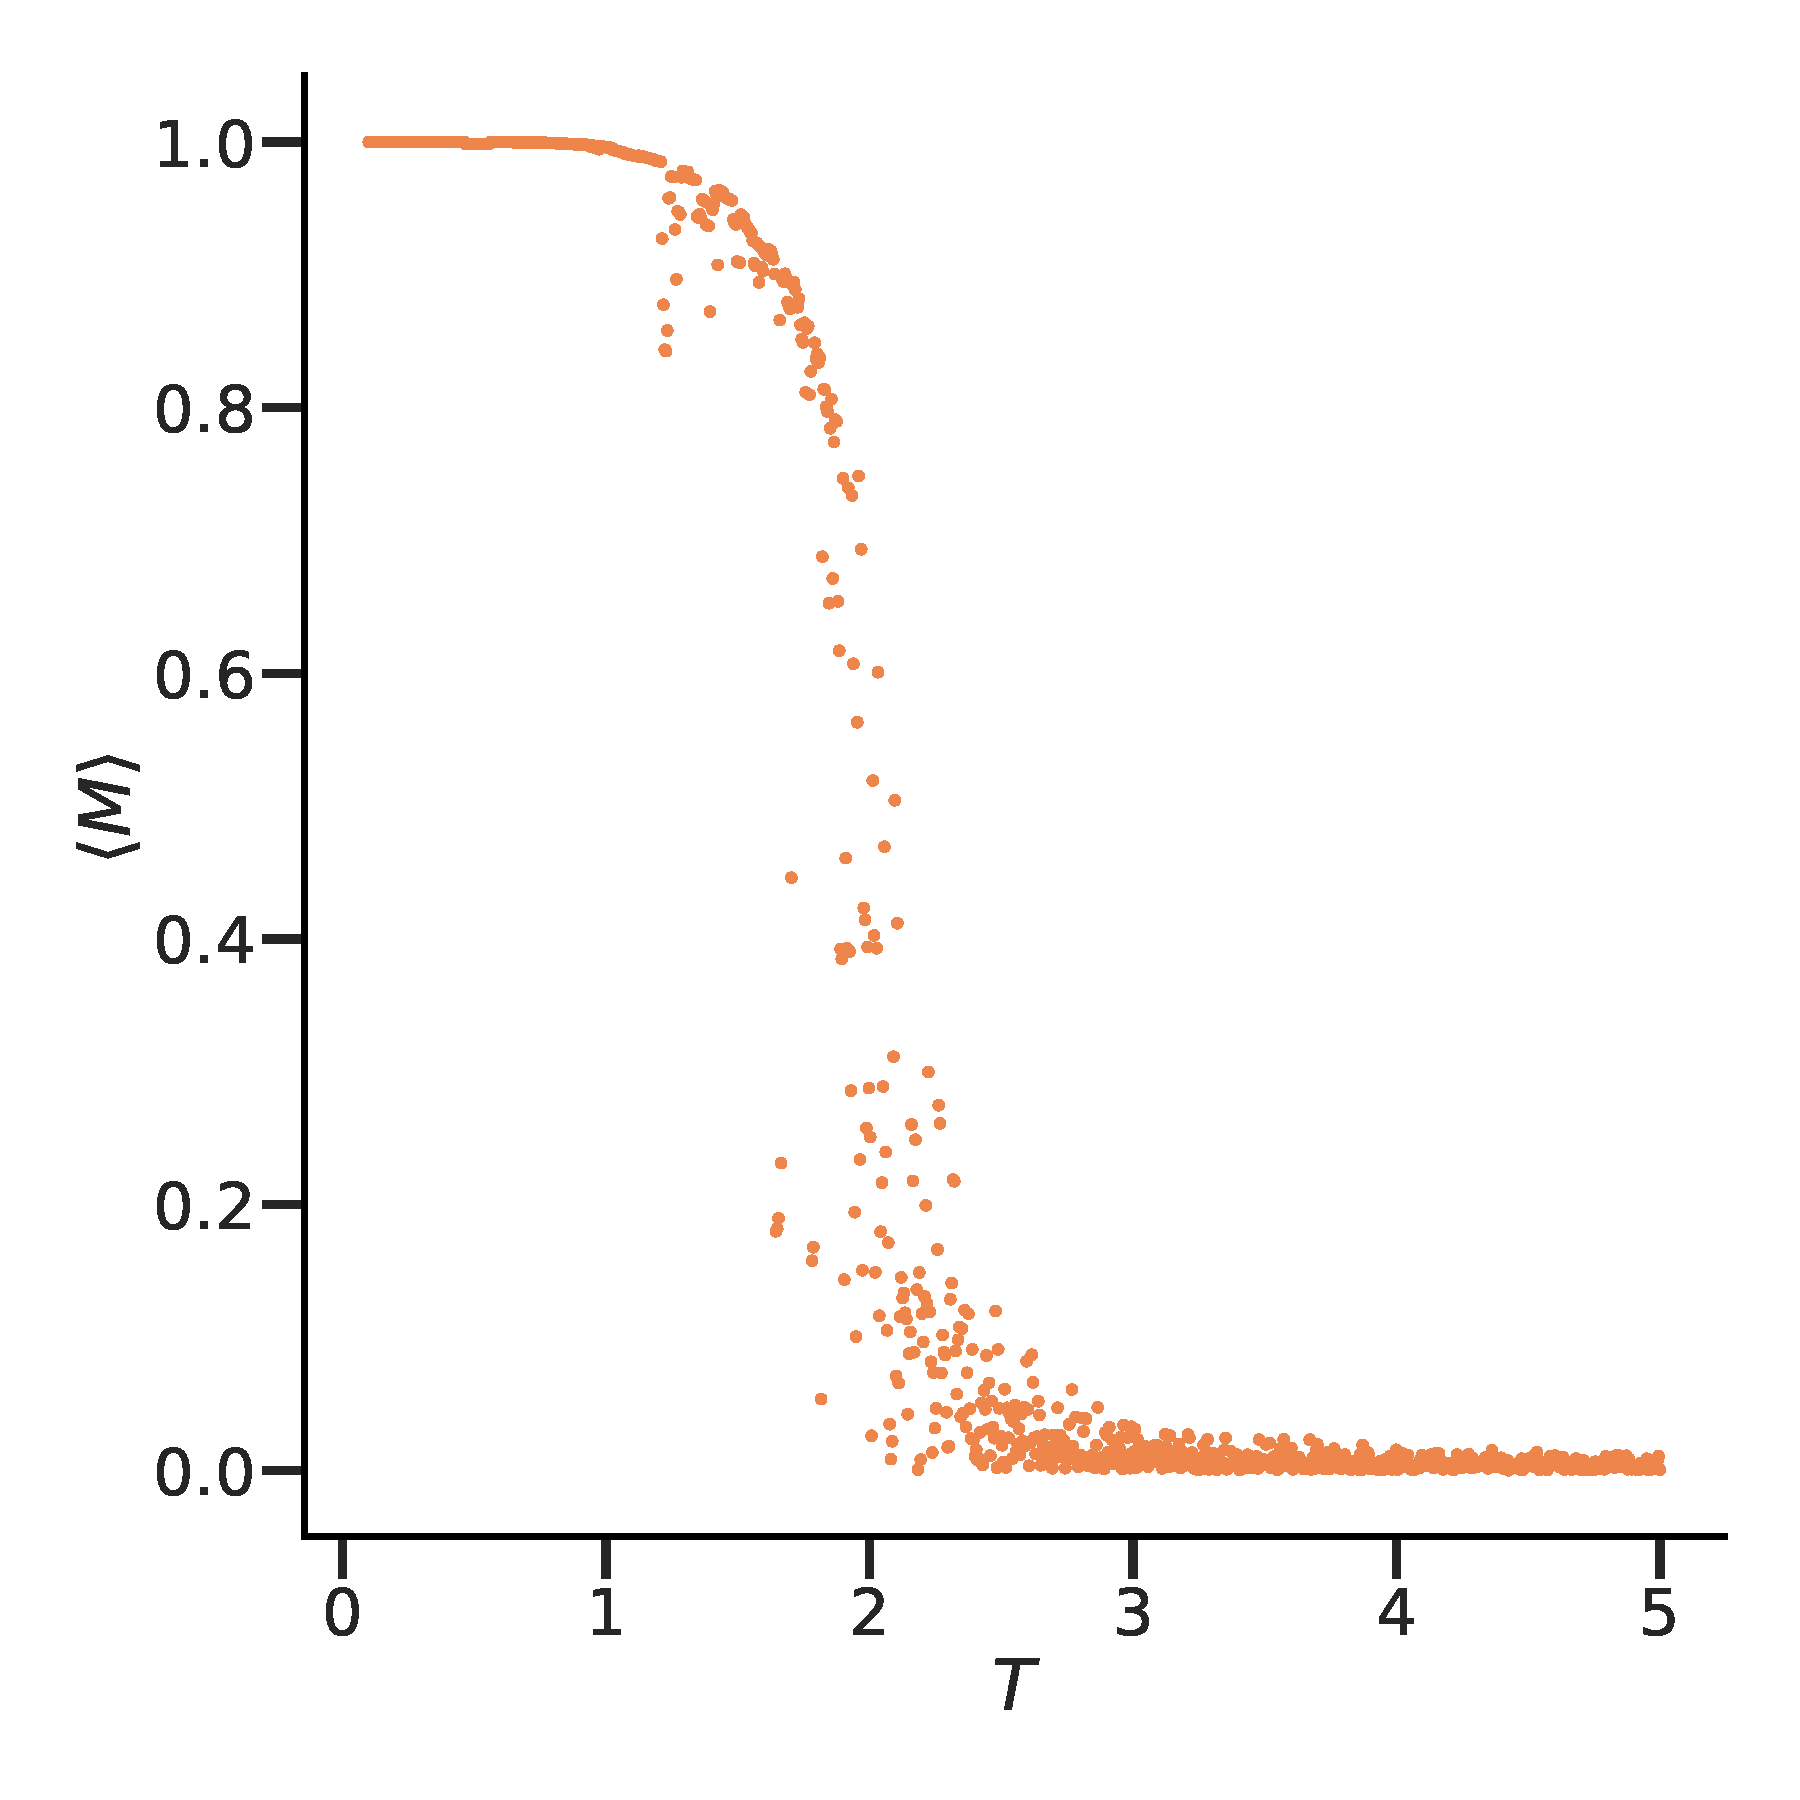
\includegraphics[width=0.6\textwidth]{../Python/mag.pdf}

        \caption{Absolute value of average magnetization as a function of temperature for a $12 \times 12$ lattice.}
        \label{fig:mag}
    \end{figure}

    \begin{figure}
        \centering
        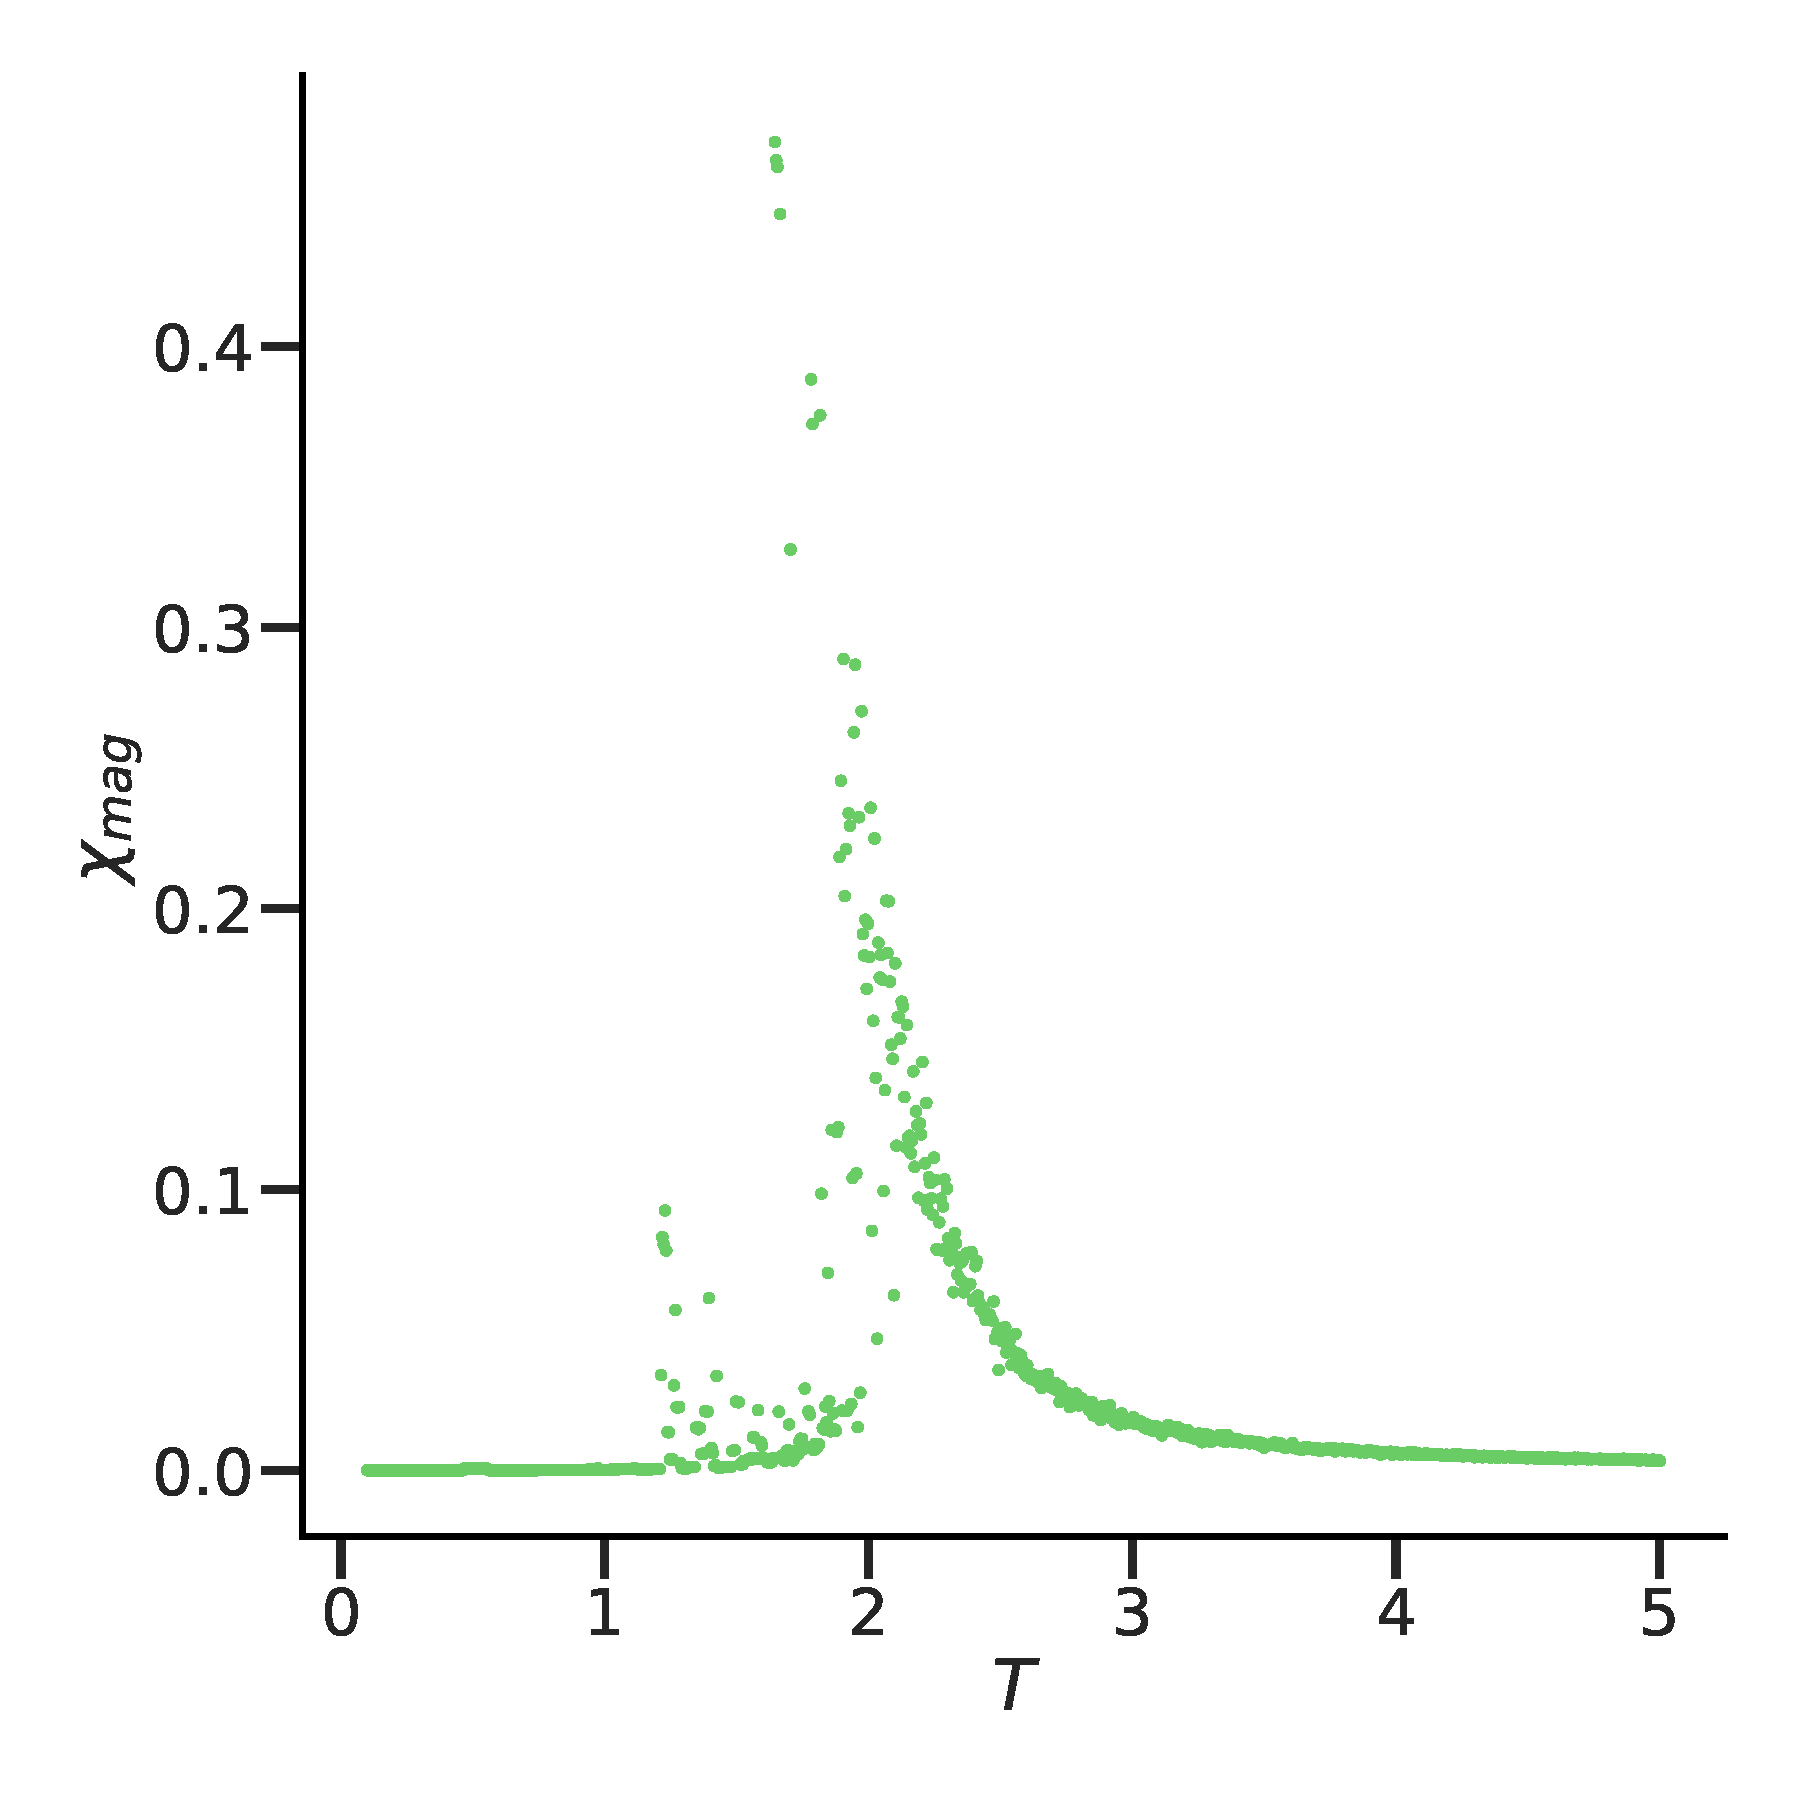
\includegraphics[width=0.6\textwidth]{../Python/mag_sus.pdf}

        \caption{Absolute value of average magnetization as a function of temperature for a $12 \times 12$ lattice.}
        \label{fig:mag_sus}
    \end{figure}

    The phase-transition is also apparent in the average magnetization~(Figure~\ref{fig:mag}), $\langle M \rangle$,
    of the system, which collapses to zero at $T_c$, indicating the emergence of a new phase in the system. This is also
    observed in the magnetic susceptibility (Figure \ref{fig:mag_sus}), computed as
    \begin{align*}
        \chi_{mag} = \frac{1}{k_b T}\left(\langle M^2 \rangle - \langle M \rangle^2)\right).
    \end{align*}

    \newpage

    \section*{N-state Ising}
    In this section, we extend the Ising model to an arbitrary number of states.
    The interaction, $J(s_1, s_2)$, and field, $B(s)$, energies are now represented a functions of the states, $\simga$,
    in an updated Hamiltonian:
    \begin{align*}
        H _{\{\sigma_i\}}= \sum_{\langle i,j \rangle} J(\sigma_i, \sigma_j) + \sum_i B(\sigma_i).
    \end{align*}

    Defining $J$ and $B$ as
    \begin{align*}
        &J(-1, 1) = -J_0 \\
        &J(-1, -1) = J_0 \\
        &J(1, 1) = J_0 \\
        &B(-1) = -B_0 \\
        &B(1) = B_0,
    \end{align*} results in the standard Ising model. \\


    \begin{figure}
        \centering
        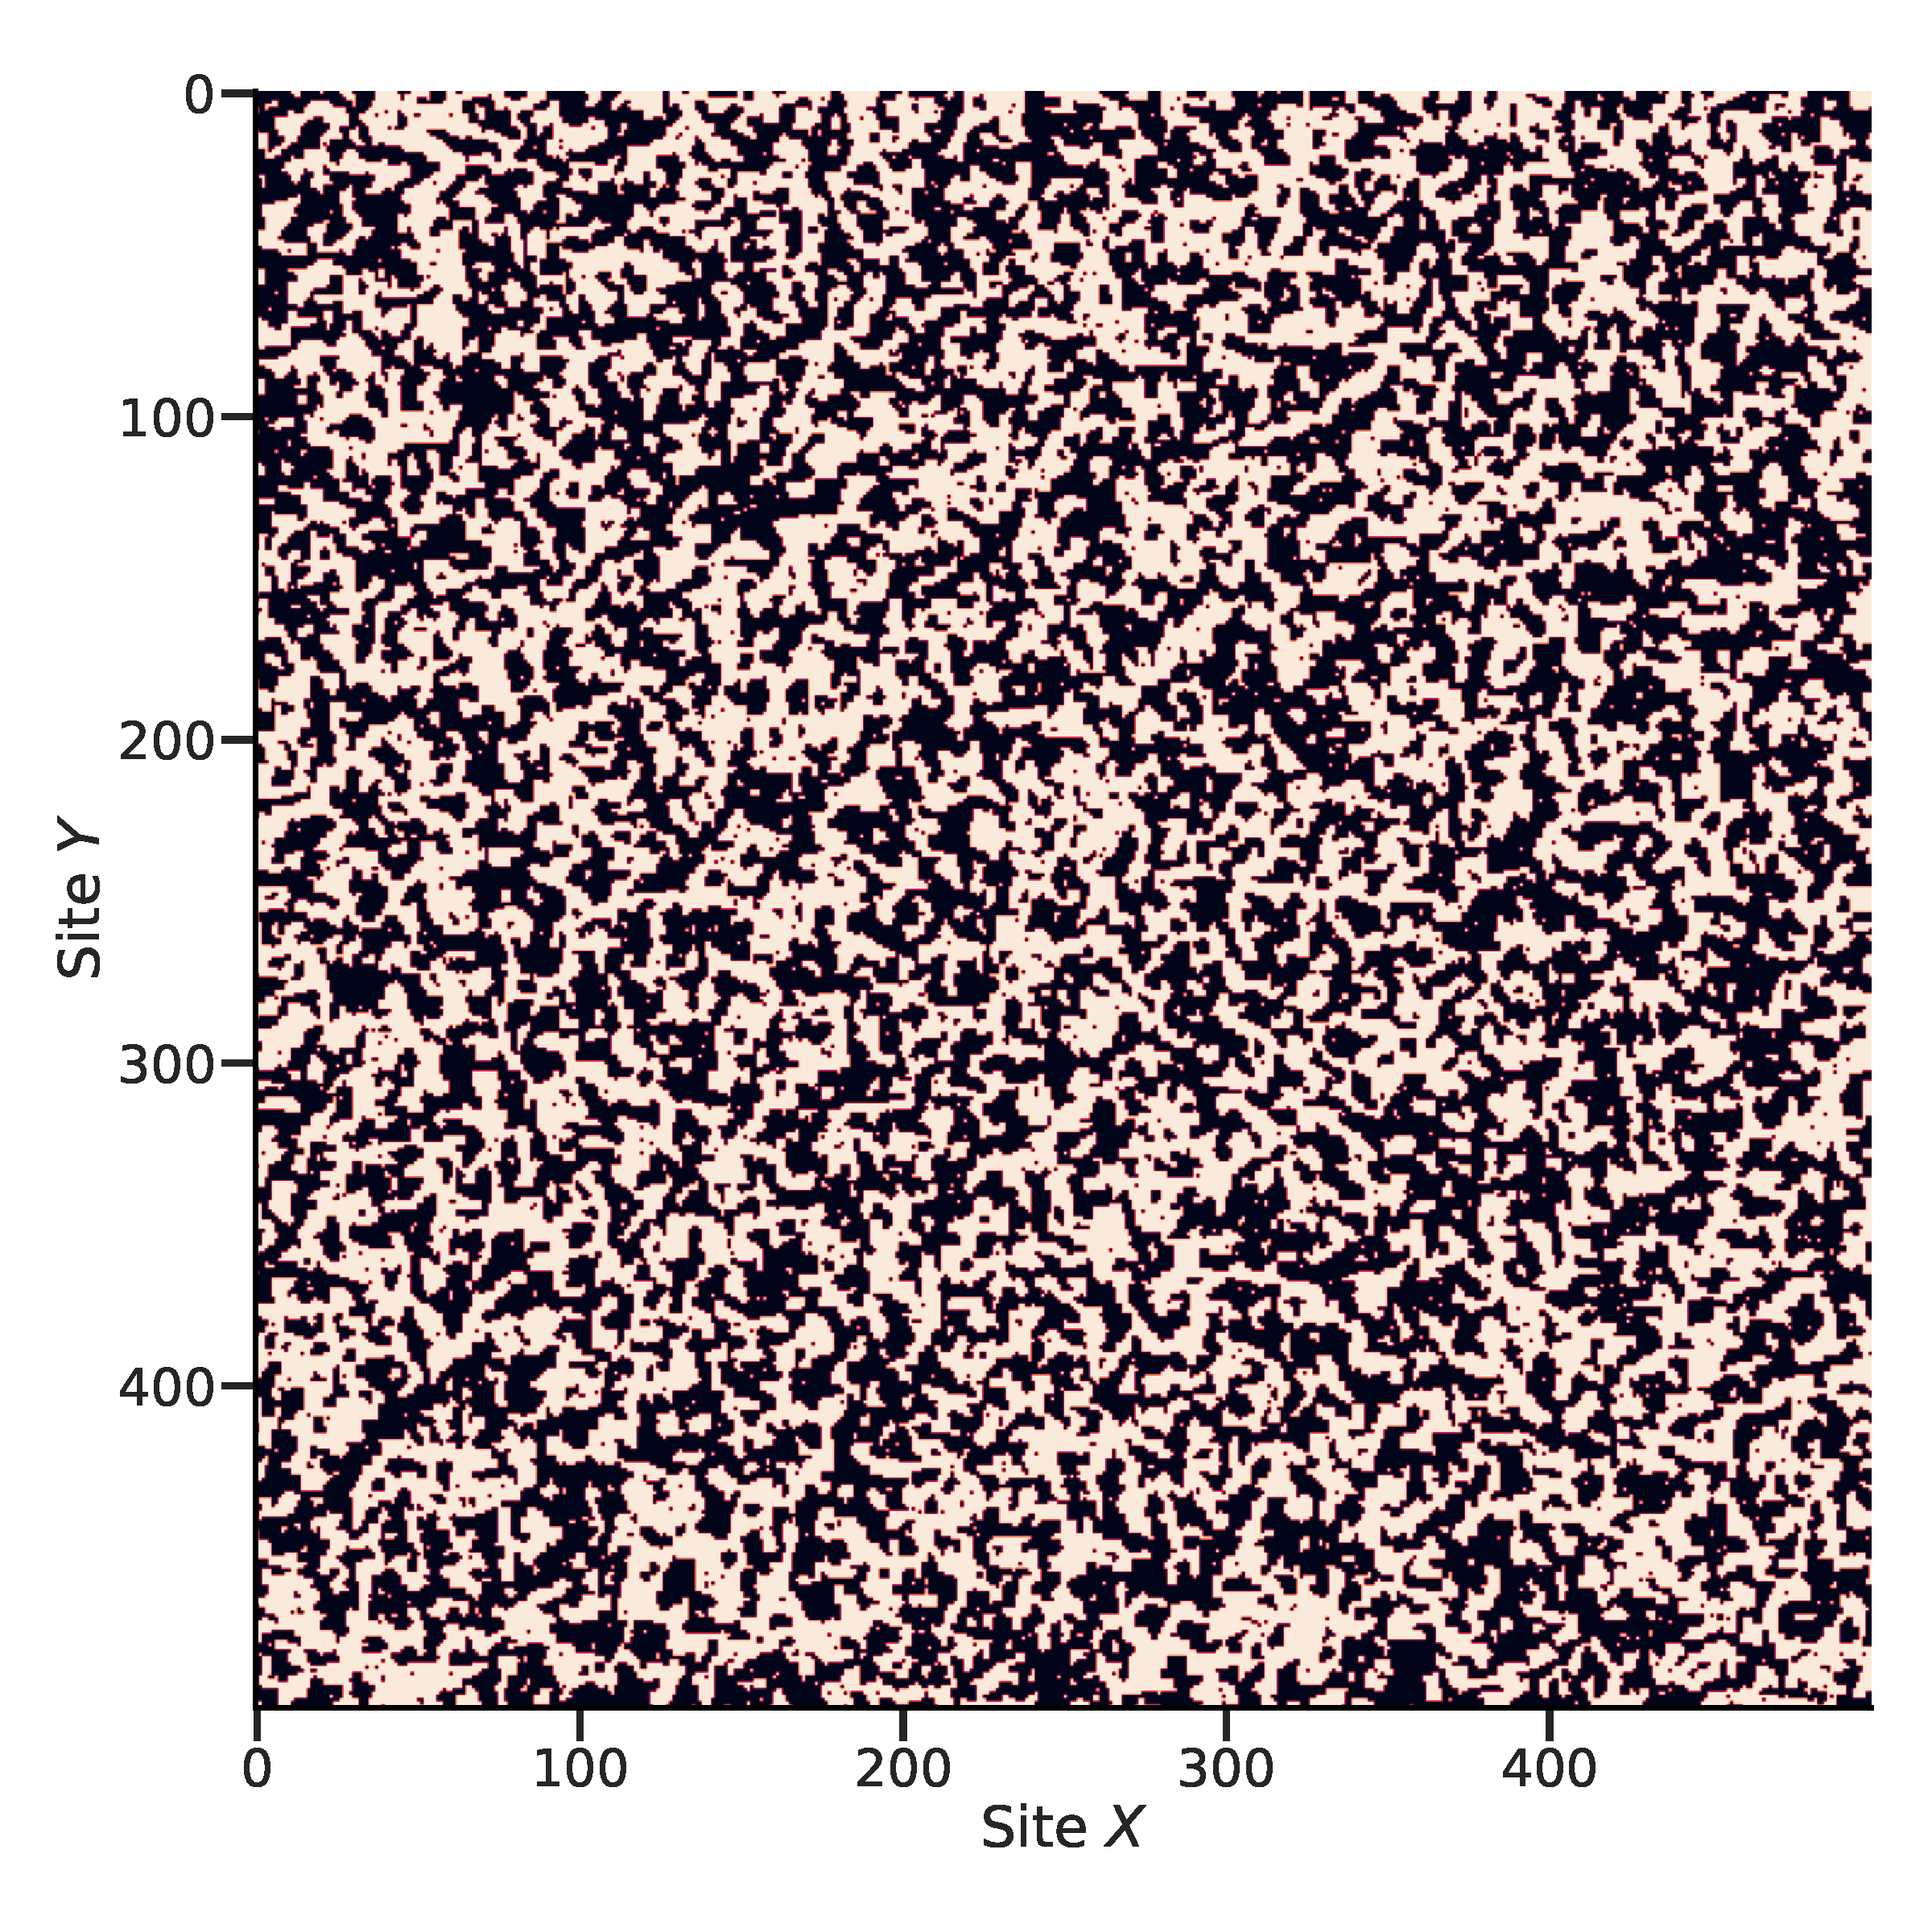
\includegraphics[width=0.6\textwidth]{../Python/grid.pdf}

        \caption{Quench of an Ising-plus-vacancy $500 \times 500$ lattice
            (Black: spin-down, White: spin-up, Red: vacancy).}
        \label{fig:grid}
    \end{figure}

    An test (Figure~\ref{fig:grid}) was run with an Ising-plus-vacancy
    ($\sigma = 0$) model, $J(0, \{-1, 1\}) = 0$ and $B(0) = 0$,
    which demonstrates this capability for the model.

    \medskip

    \printbibliography

\end{document}